\section{Orientaci\'on al arco}

Al finalizar la búsqueda de la pelota, se desea poder patearla con dirección al arco. El procedimiento para la búsqueda del arco es an\'alogo al procedimiento de la b\'usqueda de la pelota explicado en la sección \ref{sec:busqueda}.
Se tiene la representación del mundo dividida en regiones como se muestra en la figura ~\ref{divisionCamArco}. Los recuadros negros representan la imagen captada por las posiciones de la cámara (a) (c) y (e) que se muestran en la imagen de la figura ~\ref{posicionesCam}. En esta ocasi\'on se cuenta con 8 estados. Siete de ellos cuando el arco se detecta en alguna de las regiones y el último estado representa la ocasión en la que no se encuentra el arco. 

\begin{figure}[hbtp]
\centering
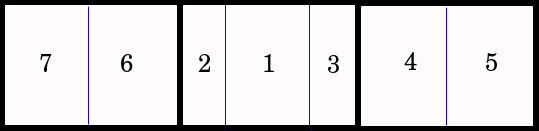
\includegraphics[scale=0.5]{imagenes/RegionesArco.jpg}
\caption{Campo de visión del robot con el número de cada región para buscar el arco. }
\label{divisionCamArco}
\end{figure}

Primero se busca detectar el arco y posicionarse frente a él intentando rodear la pelota, luego se verifica que a\'un la pelota se encuentre en la zona de pateo y se procede a patear hacia el arco.

Las acciones que se toman en cada regi\'on se especifican a continuación: 
 \begin{itemize}
\item Girar a la Izquierda: Junny debe girar a la izquierda cuando la pelota se encuentre en alguna de las siguientes regiones: 2, 6, 7.

\item Girar a la Derecha: debe girar a la derecha cuando la pelota se ubique en alguna de las siguientes regiones: 3, 4 y 5. 
\end{itemize}

Cuando el arco se encuentra en la regi\'on 1. Se da por finalizada la búsqueda y posicionamiento frente al arco.  

Los resultados obtenidos en esta tarea en particular no han sido muy favorables, pues en casos en los que el arco ya se encuentra frente al robot, este logra ajustarse con la pelota para realizar un buen tiro. Sin embargo para el rodeo de la pelota es importante poseer un grado de libertad que Junny no posee en las caderas, lo cual dificulta lograr un buen desempeño.






